\chapter{Introduction}
\label{chap:Introduction}
\section{Background}
During the early day's optimization of aerodynamics, shape optimization was a tedious job. Given a problem of drag minimization on the wing surface, the designer will manufacture the wing's prototype. Then wind tunnel testing is carried out. After looking into the results, the shape gets modified, or a new model gets manufactured. Again, subject to testing. Redesigning the wing's shape involves many resources. Even after doing all these steps, the designer ends up with a single-wing shape called a single modal design, or unimodal design optimization. With computational power and sophisticated algorithms, it is now possible to have multiple optimal shapes for an objective function subjected to constraints.

In a recent decade, computational techniques have become more reliable, assisting aircraft designers in improving the process of designing new aircraft components. Additionally, it even shortened the design cycle times and to explore higher design space effectively. For example, the CFD codes allow the designers to reduce their dependence on the more expensive and time-consuming wind tunnel tests. CFD is a mature technology that is used in every industry. High-fidelity methods provide the engineers for a better understanding of the design tradeoffs and make better decisions.

Aerodynamic shape optimization (ASO) can become a promising area of research and lead to a breakthrough in aircraft components design. This approach involves using optimization algorithms in combination with the CFD solver and the parameterization technique to reduce the problem's dimension.  These tools allow for robust tuning of the existing design. The goal of ASO is to improve the aerodynamic characteristics of the aircraft, resulting in increased fuel efficiency. 

\section{ADODG}
Despite researching more than two decades, there is no clear idea of the problem formulations used to obtain practical aerodynamic designs, and the strategies to solve aerodynamic shape optimization problems. Further,    performing the ASO based on the Reynolds-averaged Navier-Strokes (RANS) equations on a large cluster of the grid size remains challenging.  Several forums have established to compare the CFD algorithms that enable researchers to validate their codes. The aerodynamic design optimization community makes a similar attempt to initiate the AIAA Aerodynamic Design Optimization Discussion Group (ADODG).  The first meeting for the discussion group was in the year 2014.

To understand the aerodynamic shape optimization in the better way, the ADODG has developed a series of benchmark problems ranging from 2-D airfoil optimization on the Euler equations to the 3-D wing shape optimization based on the RANS equations.  These benchmark cases mainly concentrate on drag minimization subjected to several constraints.

\begin{table}
    \centering
    \begin{tabular}{m{0.1\textwidth}>{\centering}m{0.04\textwidth}>{\centering}m{0.62\textwidth}>{\centering\arraybackslash}m{0.11\textwidth}}\hline
    \textbf{Figure} & \textbf{Case} & \textbf{Description} & \textbf{References} \\\hline
    \center{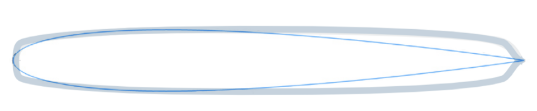
\includegraphics[width=20mm, height=8mm]{figures/case_1.png} }    & 1 & Sectional optimization of a modified NACA 0012 airfoil at zero angles of attack in inviscid, transonic flow. & \cite{case_60,case_1b,case_49}\\\hline
    \center{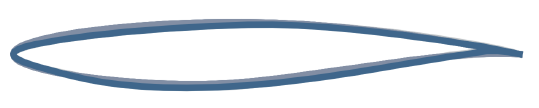
\includegraphics[width=20mm, height=8mm]{figures/case_2.png} }     & 2 & Sectional optimization of an
RAE 2822 airfoil in viscous, transonic flow. & \cite{case_60,case_1b,case_44,case_46} \\\hline
    \center{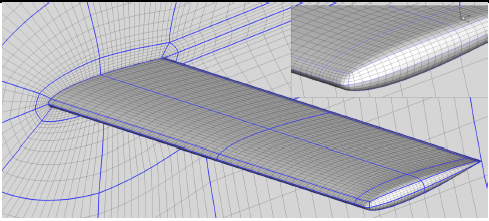
\includegraphics[width=20mm, height=10mm]{figures/case_3.png} }     & 3 & Twist optimization of a rectangular wing in subsonic, inviscid flow. & \cite{case_44,case_46,case_49}\\\hline
    \center{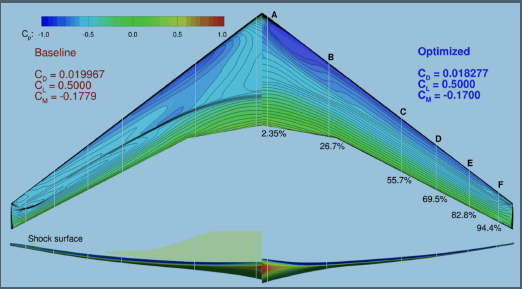
\includegraphics[width=20mm, height=10mm]{figures/case_4.png} }     & 4 & Sectional and twists optimization of the Common Research Model (CRM) wing in transonic,
viscous flow. & \cite{case_44,case_46,case_49,case_60}\\\hline
    \center{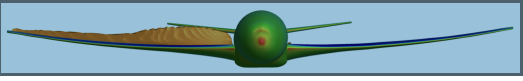
\includegraphics[width=20mm, height=10mm]{figures/case_5.png} }     & 5 & Lift-constrained drag minimization of the CRM wing-body-tail configuration at flight Reynolds number. & \cite{case_60,case_62}\\\hline
    \center{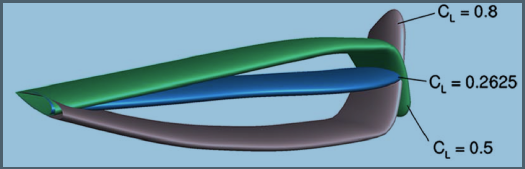
\includegraphics[width=20mm, height=10mm]{figures/case_6.png} }     & 6 &\textbf{ Multimodal subsonic inviscid lift-constrained drag minimization.} & \cite{case_63,case_64}\\\hline
    \end{tabular}
    \caption{ADODG benchmark cases}
    \label{adodg cases}
\end{table}

The benchmark cases \cite{adodg} are listed in Table \ref{adodg cases}. The objective of the problems is to minimize the drag coefficient. Most of the mentioned cases are subjected to lift coefficient constraints along with thickness constraints. Furthermore, in some cases, the problem is also subjected to moment coefficient constraints.

The first two cases are related to airfoil shape optimization benchmark problems: Case 1 begins with NACA 0012 airfoil as a baseline, whereas in Case 2, it begins with RAE 2822 airfoil. Apart from this, both the case problem solve different aerodynamic models; that is, Case 1 deals with Euler equations, and the counterpart with RANS equations. Furthermore, Case 1 does not involve the lift constraint, whereas the other does. Based on historical work available, it can be concluded that much work is carried out on this case problem. The reason for this could be the lower cost of solving the two-dimensional cases.

Cases 3 and 4 involve optimizing the wing shapes; Case 3 is a subsonic case-solving Euler equation, while Case 4 is a transonic case based on RANS. Case 3 optimizes only twist, but Case 4 includes both twist and airfoil shapes. All wing optimization cases are subjected to a volume constraint, where any optimized wing generated should posses the volume, which is higher than the baseline wing. 

Case 5 is the extension of Case 4, which adds the fuselage and tail. The baseline shape for Case 4 is the wing from the CRM full aircraft configuration combined with the fuselage intersection. Case 5 restores the full CRM aircraft configuration and is considered as a benchmark case that suits for industrial needs. Also, it uses the flight Reynolds number for testing. The thickness constraint prevents the thickness of the optimized shape, lowering below the baseline aircraft shape. Its tail rotation angle is considered another design variable used to trim the aircraft at various flight conditions.

Finally, Case 6 is a benchmark case for multimodality. More preciously, Case 6 is the wing optimization problem that is similar to Case 3 combined with the airfoil shape variables and planform variables (Sweep, span, dihedral, and chord variation). Case 6 provides additional flexibility for design space exploration and determines the existence of multimodality. 

The present work concentrates on Case 6: Multimodal optimization of the wing surface. It involves several geometric and aerodynamic constraints, which will be detailed in chapter \ref{parameterization}. Also, the problem of interest involves parameterizing the wing, choice of CFD solver, and optimization algorithm. Each of these crucial steps is explained in detail in subsequent chapters. However, a minor introduction is provided in the following sections.

\section{Importance of parameterization }
Several approaches to the parameterization of wing profiles are available in the literature. Point clouds can describe 2-D airfoils as it is done in most airfoil libraries. The number of parameters is twice the number of points (x and y coordinates); in the case of 3-D, the parameters will be thrice as that of the number of coordinates. It is undoubtedly impossible to optimize the object using the coordinate points. Parameterization allows a larger design space to represent the given object.

Methods like Radial basis function, B-splines, CST function are generally used techniques to parameterize the given object. Radial basis function methods use basis function to represent the object. The B-splines method is considered to be easy to implement for a 2-D object. Similarly, for a 3-D surface, bezier surfaces are used to parameterize the surface. CST function involves a higher degree of computation to get the perturbed coordinates back. Among all the above methods, researchers generally prefer to opt for the B-spline methods, due to its ease of implementation. Apart from these, there are methods like NURBS (Non-Uniform Rational B-spline), PARSEC, Hicks-Henne bump function, to name a few.

However, in this work, an extended version of the B-spline method called Free-form deformation (FFD) box is used. In this method, the object is circumvented using the box, and corner (control) points coordinates are used to parameter the object. Irrespective of object shape, the FFD can be implemented. FFD method uses Bernstein polynomial to parameterize the object. More on this will be covered in chapter \ref{parameterization}.
\section{Solver selection}
While address the aerodynamic shape optimization problem, the crucial step in the entire process is the choice of CFD solver. The advancement in computational power paved the way for researchers to build the solver, which is robust, open-source, portable, and efficient in their performance. Further, the CFD solver is expected to satisfy the practical industrial constraints. In the present condition, the solver is combined with several ASO supporting modules, namely gradient calculation, mesh deformation, grid generation, to name a few. These solvers are generally written in C++ modules for ease of readability.

The work presented here uses SU2 as the CFD solver. The choice behind the solver is its ease in the implementation, open-source, portability, and, more importantly, it is embedded with the FFD box. Python modules are used to build a SU2 solver. This further increases its reach into the optimization problems. Also, it possesses the gradient calculation and a full-fledged optimizer, which does the entire design step. Since the present work demands the inviscid (Euler) equation to solve, the selected CFD solver is sufficient for use.

\section{Choice of optimizer}
Optimization is a computationally expensive process. A unique optimization algorithm cannot address all the optimization problems. Finding a suitable algorithm is problem-dependent. Also, it depends on the number of constraints, type of design variables, to name a few.

Based on constraint availability, an optimization problems is classified into Constraints optimization problems (COP), and Unconstrained optimization problems (UOP). Most of the real-world problems are COP. However, UOP is worth studying because COP can be converted into UOP using a penalty approach. In addition to this, an optimization problem can have discrete design variables or integer design variables.
However, in a broader sense, optimization methods is classified two categories:
\begin{itemize}
\item Gradient-based (GB) method.
\item Gradient free method.
\end{itemize}

The Gradient-based (GB) algorithm involves finding the gradient [appendix \ref{gradient_vector}] at every iteration. For example, Quasi-Newton methods, such as Broyden-Fletcher-Goldfarb-Shanno (BFGS) involves constructing a Hessian approximation [appendix \ref{Hessian_matrix}] at every iteration. The steepest-descent and the conjugate-gradient requires the calculation of first derivative of the objective function. While the others need the second derivative (Hessian matrix) of the objective function. Any function $f(x)$ can be expressed in terms of divergence and Hessian matrix which is as represented in appendix \ref{Taylor_equation}. The GB methods is generally used for higher dimensional problems.

In real-world problems, it is quite often to encounter non-differentiable problems, non-convex design space, discrete feasible space, large dimensionality functions, multiple local optima, or multiple objectives problems. These kinds of problems are not possible to address from the gradient-based method, as they involve gradient calculation, which may not be available. Under this circumstance, Gradient free methods come in handy, which do not involve any gradient calculation and are heuristic in nature. 

Many gradient-free methods are developed in the early days, like the Nelder-Mead Simplex algorithm, Simulated Annealing, Divided Rectangules Method, Genetic Algorithms, Particle Swarm Optimization, to name a few. This work concentrate on the genetic algorithms because of implementation simplicity.

\section{Comparision between Gradient-based and Gradient free methods.}
Gradient-based methods are efficient in finding local minima for problems that generally possess nonlinear constraints, higher dimensional, and convex problems\cite{stanford_university}. However, these methods have problems while dealing with noisy and discontinuous functions. Also, these methods are not designed to handle multi-modal problems or discrete-continuous design variables. Many gradient-free methods are heuristic in nature. Unlike the gradient-based method in a convex design space, the gradient-free methods may not converge to a global optimal. However, these may result in multiple good solutions rather than a single best solution.

Consider, for example, the Griewank function [\ref{griewank_formula}],
\begin{equation}
f(x)=\sum_{i=1}^{n} \left(\frac{x_{i}^{2}}{4000}\right)-\prod_{i=1}^{n} \cos \left(\frac{x_{i}}{\sqrt{i}}\right)+1 
\label{griewank_formula}
\end{equation}
\begin{equation*}-600 \leq x_{i} \leq 600\end{equation*}
\begin{figure}[!htbp]
    \centering
    \framebox{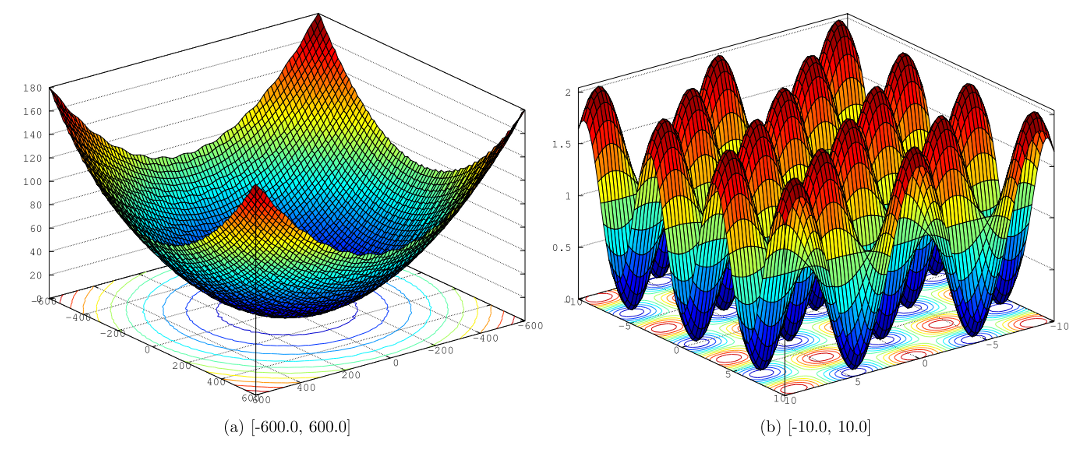
\includegraphics[scale = 0.39]{figures/griewank_image.png}}
    \caption{Griewank function for n = 2, right side image represent the domain (-600, 600), and the left side image represent the domain (-10, 10) \cite{griewank_reference}}
    \label{griewank}
\end{figure}

The Griewank function appears smooth (convex) when plotted in a broader domain (left). However, the same function plotted in smaller design space result in multiple local minima (right). Every run with a gradient-based method will converge to the nearest local minima. Further, a multi-start gradient-based method is introduced. Here the optimizer is initialized from multiple points within the design space. With this, there is a possibility of finding the global optima, But not always guaranteed for convergence to global optima. The frequency of using multi-start method is rare because,
\begin{itemize}
\item  large computational cost.
\item  No guarantee about the success of the search.
\end{itemize}

The problems which seem difficult to solve using gradient-based methods, the gradient-free method can be implemented. In addition to this, many of the gradient-free methods are designed to find global optimal. However, they can find multiple local optima while searching for global optima.

Differential evolution is a class under a genetic algorithm. These algorithms evolve with time, which implies the solution move to the optimal point after every generation. These algorithms follow mutation, crossover, and selection phases. However, implementing the DE will not result in obtaining the multimodality. So the modified form of the DE algorithm has to be used. These modifications are named as niches, and the modified algorithms are called as niching algorithms. More on this is explained in chapter \ref{niching}.

This work constitutes finding multiple optima. On considering above mentioned methods, the gradient-free method/optimization (specifically genetic algorithm) align better with the present work. Furthermore, the implementation is straightforward and easily parallelized.

\section{Outline}
This thesis is divided into six further chapters,
\begin{itemize}
\item Chapter \ref{literature} provides information about the literature review related to problem mentioned in ADODG Case 6, parameterization of wing, and selection of optimizer.
\item Chapter \ref{niching} describes the differential evolution based niching algorithm. Furthermore, this chapter contains several niching algorithms that are implemented over the test function. This chapter concludes by selecting one of the niching algorithms used in this work to implement the ADODG Case 6 problem. 
\item Chapter \ref{parameterization} explains the parameterization of the wing surface. It includes a detailed explanation of the FFD box, followed by the PCA implementation. Furthermore, the chapter concludes by mentioning the problem dimension after the FFD box and PCA method. 
\item Chapter \ref{solver} mention the choice for CFD solver and the parameter used to set up the CFD solver. Additionally, it describes the parameters involved in job submission into the HPC cluster via SLURM. 
\item Chapter \ref{methodology} deals with the flow of data right from the baseline geometry until the end of optimized wing shapes. It contains the equation to generate the NACA 0012 airfoil, extruding the 2-D airfoil to 3-D wing, implementation of the FFD box, and PCA method, creating the winglet, followed by the SU2 solver implementation. The flow chart representing the flow of data is presented. Along with this, this chapter even mentions about the glyph script, which creates the wingtip, followed by creating volume mesh and setting boundary conditions. 
\item  Final chapter \ref{results} details the test function results and also the results associated after optimizing the wing. Further, it explains the conclusion and highlights the scope for future work. 
\end{itemize}
